\documentclass[10pt]{article}
\usepackage[utf8]{inputenc}
\usepackage[shortlabels]{enumitem}
\usepackage[margin=1in]{geometry}
\usepackage{setspace}
\usepackage{hyperref}
\usepackage{graphicx}
\usepackage{natbib}
\usepackage{booktabs}
\usepackage{subcaption}
\onehalfspacing
\setlength{\parskip}{1em}
\setlength{\parindent}{0pt}
\bibliographystyle{ecta}
\usepackage[T1]{fontenc}
\usepackage{titling}
\usepackage{amsmath}
\setlength{\droptitle}{-7em}
\addtolength\abovedisplayskip{-3in}
\addtolength\belowdisplayskip{-3in}

\title{City Location Choice and Household Productivity}
\author{Tan Sein Jone}
\date{\today}

\begin{document}
\doublespacing
\maketitle

\vfill

\begin{abstract}
    This paper develops a novel model of city location choices by extending the framework of \cite{lindandramondo} to an urban context, explicitly incorporating occupations as distinct nests. By leveraging a two-stage least squares regression with a shift-share instrument, I estimate key parameters and explore the dynamics of within-occupation migration. My analysis of American Community Survey data reveals significant insights into the role of occupational composition in shaping migration patterns. Counterfactual simulations further illustrate how shocks to specific cities and occupations influence household relocation, emphasizing the importance of city-specific occupational structures. My findings offer valuable implications for urban policy design and the optimization of place-based interventions.
\end{abstract}

\vfill

\noindent\textbf{Keywords:} Quantitative Spatial Models; Urban Economics; Comparative Advantage; Migration; Agglomeration

\vfill

\newpage

\section{Introduction}

Cities capture a disproportionate amount of household location choices worldwide. In 2018, 55\% of the world's population lived in urban areas, and this is expected to increase to 68\% by 2050. This trend is driven by the benefits cities provide, such as access to jobs, amenities, and social networks. While these advantages are often considered universal to all households, regardless of their occupation-specific skills, the benefits of each city clearly vary for different households. For instance, an auto worker from Detroit will not view New York as an equivalent substitute for a city to live in compared to a finance worker from New York. Given the billions of dollars spent on place-based policies, it is crucial to understand this dimension of absolute advantage, where a city can provide higher levels of productivity for households working in specific occupations.

Forces of spatial inequality and agglomeration have been well documented in the literature (\cite{behrens2014}; \cite{br2015}), showing that large, dense cities have higher levels of productivity, resulting in higher wages. These cities, however, tend to attract households with specific skills, reflected in the occupational composition of the cities. As seen in \cite{lagakos_waugh2013}, households will self-select into occupations where they are most productive. In large cities, these are often occupations that disproportionately benefit from the amenities of dense urban areas. This effect is also seen in smaller cities specializing in occupations such as farming, where households particularly productive in those occupations choose to live. One benefit of this self-selection is the co-location with households who are also productive in that occupation, leading to knowledge spillovers. \cite{dandd} show that the exchange of ideas plays an important role as an agglomeration force in cities. Besides occupations, education has also been documented as an important factor in sorting. Even within a given city, highly educated households tend to live in areas of high productivity and wages (\cite{diamond}; \cite{diamond2022}).

A city's absolute advantage exists in three dimensions. First, there is a city-specific advantage that makes all occupations more productive in that city, primarily due to its size and population, resulting in better amenities, more jobs, and a larger social network. Second, there is an occupation-specific advantage that is universal across all cities; some jobs are simply more productive than others, and cities specializing in these jobs will be observed as having higher overall choice shares of households. Third, there is a city-occupation-specific advantage, where a city may have specific policies that make it more attractive for a particular occupation, such as tax breaks for mechanics in Chicago. It is crucial to distinguish between occupations and sectors: sectors employ broad categories of jobs (e.g., manufacturing, services, agriculture), while occupations are specific jobs (e.g., mechanic, clerk). Cities can specialize in occupations by focusing on sectors that intensively use those occupations.

In this paper, I propose a model of city location choices based on a class of models in the quantitative trade literature first proposed by \cite{ek}. These models treat productivity as random draws from Fr\'{e}chet distributions, allowing for non-zero production of goods, which helps account for small cities. \cite{redding} applies this model to an urban setting by loading city heterogeneity onto amenities, capturing the first dimension of absolute advantage. However, both these models rely on the independence assumption, which treats goods and cities as perfect substitutes for each other. \cite{lindandramondo} break this assumption by introducing a nested CES utility structure, allowing for correlated draws of productivity within nests across countries. I apply this structure to the urban setting by treating occupations as independent nests, capturing substitution patterns where cities with similar occupational structures are treated as better substitutes for each other. This approach enables us to capture all three dimensions of absolute advantage.

My model is part of the larger class of quantitative spatial models as proposed by \cite{redding2017}, with modifications that allow us to capture the effects of trade shocks at the group level, similar to the work of \cite{galle2023}. As shown by \cite{adh2013}, trade shocks have heterogeneous effects on industries with differing exposure to trade shocks, leading to sharp movements in wages but slow adjustments in labor market outcomes (\cite{acm2010}). I will be able to capture these effects in counterfactual exercises once I have estimated the parameters of my model. Given my class of models, I will be able to draw from techniques and estimations already existing in the literature, such as \cite{albert_monras2022}, who estimate migration elasticity, and \cite{kim_vogel2020}, who estimate the elasticity of labor market adjustments to trade shocks. I also make use of shift-share instruments (\cite{bartik1991}), specifically shifts in total factor productivity for industries with different shares of occupations, that are widely used in the trade literature to estimate my parameters. This approach will require us to base my identification on either exogenous shares (\cite{pssh2020}) or exogenous shifts (\cite{bhj2020}).

In the first section, I adapt the model of \cite{lindandramondo} to the urban setting, explicitly modeling occupations as nests, unlike their original paper where nests are implied. This specification yields several implications:

\begin{enumerate}
    \item I can observe both overall city shares and city shares specific to each occupation, as well as city occupation compositions, which serve as a measure of similarity between cities.
    \item Using this data, I derive elasticities for three dimensions of absolute advantage: city-specific, occupation-specific, and city-occupation-specific. The last elasticity serves as a sanity check for the direction of substitution, while city and occupation elasticities verify my claim of unbalanced substitution patterns favoring similar cities. In other words, shocks to cities with a certain occupational composition will have larger effects on cities with similar compositions due to correlations in productivity draws.
\end{enumerate}

The second section presents my estimation strategy. I exploit variation over time to recover an important parameter of mymodel: the correlation parameter $\rho$, which determines within-occupation migration patterns. I use previously estimated parameters of across-occupation migration elasticity $\theta$ from \cite{redding}. This process also allows us to recover my city, occupation, and city-occupation-specific shifters.

In the third section, I apply my estimation equations to data from the American Community Survey at the metropolitan area and occupational level. I begin by presenting stylized facts about cities and their compositions, comparing similarities among top cities. I then discuss my estimation results, focusing on the correlation parameter $\rho$ and my city, occupation, and city-occupation-specific shifters. As I will demonstrate, $\rho$ can be interpreted as the degree of within-occupation migration, while $\theta$ represents the degree of across-occupation migration.

Using this fully calibrated model, I conduct counterfactual analyses and simulate the effects of shocks at both the city and occupation levels. This analysis allows us to evaluate the effectiveness of place-based policies and provide recommendations for designing such policies to maximize their impact.

\section{Model}

\begin{align*}
    Y_{ck} = Z_{ck}
\end{align*}

Consider a closed economy consisting of $N$ cities and $K$ occupations. Each city $c$ employs households in occupation $k$ to produce output $Y_{ck}$. I assume no trade costs between cities and that the price of the good produced is freely traded and priced under perfect competition. The price index of city $c$ is given by $\Phi_c$ and the wage of a household living in city $c$ working in occupation $k$ is given by $w_{ck} = \Phi_c Z_{ck}$ where $Z_{ck}$ is the productivity of the household. I assume that when a household chooses to work in a particular occupation, they will be randomly allocated to a sector within a given city. A household has symmetric CES preferences over cities and occupations and will choose a city-occupation pair that maximizes their utility. I will assume that households are perfectly mobile across cities and that there are no fixed costs to moving. The productivity of a household within a given city-occupation is drawn from a Fr\'{e}chet distribution. In \cite{ek}, the Fr\'{e}chet distribution is used to model productivity draws in a trade setting and has two main components. The shape parameter $\theta$ which determines the dispersion of draws across the distribution and reflects the heterogeneity of cities. $\theta$ will also determine the gains from city choices, ie how much households will gain from having more choices of cities to live in, which is analogous to gains from trade. The scale parameter $T_{ck}$ is a level shifter that determines the absolute advantage of a city-occupation pair, reflecting its attractiveness. My specification so far assumes independent draws of productivity across cities, the joint distribution of which is given by:

\begin{align*}
    P[Z_1 < z_1, \dots, Z_N < z_N] & = \prod_{c}^{N} P[Z_c < z_c]                                 \\
                                   & = \exp \left\{ - \sum_{c}^{N} T_{ck} Z_c^{- \theta} \right\}
\end{align*}

This result implies that the choice shares of households for a given city is equal to the probability of households choosing that city. So far, I have stuck with the the base EK specification with the only modification being the mapping of productivity onto wages rather than prices which allows us to obtain city choice shares. I will now abandon the independence assumption and introduce a structure that allows for correlated draws across cities.

\begin{align*}
    P[Z_1 < z_1, \dots, Z_N < z_N] = \exp \left\{ - \left( \sum_{c}^{N} (T_{ck} Z_c^{- \theta})^{\frac{1}{1 - \rho}} \right)^{1 - \rho} \right\}
\end{align*}

Notice with this structure that the shape of the distribution is no longer purely determined by $\theta$ but also by the correlation parameter $\rho$. Where the distribution of productivity within a given occupation decreases as $\rho$ increases. Meaning that within a given occupation, the higher correlation will result in cities being more similar with each other in terms of productivity. When $\rho = 0$, the distribution reduces down to the original joint distribution with the shape being purely determined by $\theta$ and where draws are independent. As $\rho \rightarrow 1$, the draws become perfectly correlated and the productivity is identical across all cities.

\subsection{Cross Nested CES}

\begin{align}
    P[Z_1(\nu) < z, \dots, Z_N(\nu) < z] = \exp \left\{ - \sum_{k}^{K} \left[ \sum_{c}^{N} (T_{ck} Z_c^{- \theta})^{\frac{1}{1 - \rho_k}} \right]^{1 - \rho_k} \right\}
\end{align}

I will assume that productivity is distributed max stable multivariate Fr\'{e}chet with $T_{ck}$ being the scale parameter for city $c$ and occupation $k$. $\theta > 0$ is the shape parameter that determines the dispersion of draws across the distribution and $\rho_k$ is the occupation specific correlation parameter. As in \cite{lindandramondo}, I adopt a cross nested CES structure with a correlational structure within independent occupational nests. This has the characteristic of distributions not purely determined by $\theta$ but also by the correlation parameter. This is because the correlation parameter determines the degree of correlation between draws of productivity across cities.

In order to identify the three dimensions of absolute advantage, I will be separating out the scale parameter into three components where $T_{ck} = T_c T_k t_{ck}$. $T_c$ is the city specific scale parameter which captures the attractiveness of a city, shifting the distribution of all productivity draws within that city upwards. $T_k$ is the occupation specific scale parameter which is common across all cities, this captures the effect that any occupation has across all cities. $t_{ck}$ is the city-occupation specific scale parameter which captures the effect of a city on a specific occupation. This will give us the final dimension of absolute advantage.

\begin{align*}
    Z = \max_c \left\{ \frac{Z_c}{\Phi_c} \right\}
\end{align*}

A household's schedule of productivity is characterized by a vector of draws from different Fr\'{e}chet distributions for each city occupation pair. The realized productivity a household has in city $c$ is the occupation that maximizes the productivity has in the city. Unlike sequential games where households might pick a city before picking an occupation, I assume that households pick both simultaneously. A way to contextualize this is to think of households as already having an ideal occupation in mind when picking a city, hence $Z_c = \max_k \left\{ Z_{ck} \right\}$. This productivity is then scaled by the price index of a city to reflect how high prices reduces the purchasing power of the household within that city, hence making it less attractive.

% \subsection{Household Problem}

% \begin{align}
%     \max_{c, k} \left\{U(\nu) = \frac{y(\nu)}{\Phi_c} \right\}
% \end{align}

% Now assume that the economy has households of type $\nu \in [0, 1]$ who earn an income $y(\nu)$. The household's utility is given by the ratio of income to the price index of the city. Each household will simultaneously choose a city occupation pair that maximizes their utility. Given that all goods are traded freely and all firms operate in perfect competition, I will make the assumption that all cities will have a common price index $\Phi_c = \Phi$. This will allow us to simplify the household's problem to the following:

% \begin{align*}
%     \max_{c, k} \left\{U(\nu) = \frac{L(\nu) w_{ck}(\nu) Z_{ck}(\nu)}{\Phi} \right\}
% \end{align*}

% where $y(\nu) = L(\nu) w_{ck}(\nu) Z_{ck}(\nu)$, $L(\nu)$ is the portion of time dedicated to labor, $w_{ck}(\nu)$ is the wage of the household in city $c$ working in occupation $k$, and $Z_{ck}(\nu)$ is the productivity of the household in city $c$ working in occupation $k$. I will now assume that households spend all their time working $L(\nu) = 1$ and that the wage is the only source of income. Expanding $w_{ck} = T_c T_k t_{ck}$, I wil get the final household maximization problem.

% \begin{align*}
%     U^{\star}(\nu) = \max_{c, k} \frac{1}{\Phi} \left\{T_c T_k t_{ck} Z_{ck}(\nu) \right\}
% \end{align*}

% Here, I can see that the household maximization problem is separated into two components. The first being the expected wage which households will receive in a given city-occupation pair, determined by the scale parameters $T_c$, $T_k$, and $t_{ck}$. And the second is the idiosyncratic productivity draw $Z_{ck}(\nu)$ which is drawn from a Fr\'{e}chet distribution and is unique to each household type resulting in deviations from the expected choice shares. The assumption of a common price index would mean that any changes in shares of households across cities would not affect the overall price index. This results in a partial equilibrium model where changes resulting from a shock are assumed to be stable. While this is a limitation of the model, it is a necessary assumption in order to make the model tractable.

\subsection{Equilibrium}

\begin{align}
    G(Z_1^{- \theta}, \dots, Z_N^{- \theta}) = \sum_{k}^{K} T_k \left[ \sum_{c}^{N} (t_{ck} Z_c^{- \theta})^{\frac{1}{1 - \rho_k}} \right]^{1 - \rho_k}
    \label{nested_ces}
\end{align}

I first define $Z_c^{- \theta} = (\gamma)^{- \theta} (T_c)^{\theta}$ and $\gamma = \Gamma (\frac{\theta + 1 - \rho_k}{\theta})^{\frac{1}{1 - \rho_k}}$. Given mydefinition of $Z_c^{- \theta}$, $T_c$ will be absorbed within $Z_c^{- \theta}$, giving us the correlation function $G(Z_1^{- \theta}, \dots, Z_N^{- \theta})$ as defined in expression \ref{nested_ces}.

\begin{align*}
    \pi_c = \frac{Z_c^{- \theta} G_c(Z_1^{- \theta}, \dots, Z_N^{- \theta})}{G(Z_1^{- \theta}, \dots, Z_N^{- \theta})}
\end{align*}

Where $G_c (Z_1^{- \theta}, \dots, Z_N^{- \theta}) = \partial G(Z_1^{- \theta}, \dots, Z_N^{- \theta}) / \partial Z_c^{- \theta}$. The expression above gives us the city specific choice shares of households across all occupations. In order to evaluate the expression, I make the simplifying assumption that the correlation parameter is the same across all occupations $\rho_k = \rho$.

\begin{align*}
    \lambda_{k} = \sum_{c}^{N} \left( t_{ck} Z_{c}^{-\theta} \right)^{\frac{1}{1-\rho}}
\end{align*}

I introduce the above expression which measures the appeal of occupation $k$. Given that the expression does not include $T_k$, it does not capture the attractiveness of occupation $k$. Instead the expression captures the extent to which a given occupation $k$ exhibits city-specific productivities which are correlated with aggregate city-level attractiveness. The following definitions will be useful in simplifying the expression for city shares.

\begin{align*}
    \pi_{ck} = \frac{Z_c^{- \theta} G_c^k(Z_1^{- \theta}, \dots, Z_N^{- \theta})}{G^k(Z_1^{- \theta}, \dots, Z_N^{- \theta})}
\end{align*}

To obtain occupation specific choice shares, I can evaluate the derivative for city shares at the occupation level. More specifically, rather than $G(Z_1^{- \theta}, \dots, Z_N^{- \theta})$, I will be evaluating $G^k(Z_1^{- \theta}, \dots, Z_N^{- \theta}) = \sum_{c}^{N} (t_{ck} Z_c^{- \theta})^{\frac{1}{1 - \rho_k}}$. This will give us the following:

\begin{align}
    \pi_{ck} = \frac{(t_{ck} Z_c^{-\theta})^{\frac{1}{1 - \rho}}}{\lambda_k}
    \label{city_occuaption_shares}
\end{align}

Moving forward, it will be convenient for us to provide the following definitions. First, I define $\phi_{ck}$ as the absolute advantage of city $c$ in occupation $k$. This can be interpreted as an occupation's within city choice shares. As such $\phi_{ck}$ will be between 0 and 1. I define this formally as:

\begin{align}
    \phi_{ck} \equiv \frac{{t^{\frac{1}{1-\rho}}_{ck}}{T_{k}}\lambda_{k}^{-\rho}}{\sum\limits_{k}{t^{\frac{1}{1-\rho}}_{ck}}{T_{k}}\lambda_{k}^{-\rho}}
    \label{occupation_by_city_shares}
\end{align}

Second, I define an occupation specific choice share which takes into account both the size of each occupation, as measured by productivity $T_k$, and the extent to which individual city-occupation productivities are correlated with overall city attractiveness. This is defined as the following expression:

\begin{align}
    \omega_k \equiv \frac{{T_{k}}\lambda_{k}^{1-\rho}}{\sum\limits_{k}{T_{k}}\lambda_{k}^{1-\rho}}
    \label{occupation_shares}
\end{align}

From the perspective of discrete choice demand models, $\omega_k$ can be interpreted as the "market share" of occupation $k$. This is because it captures the extent to which the productivity of occupation $k$ is correlated with overall city attractiveness. The expression is normalized by the sum of all $\omega_k$ to ensure that the sum of all market shares is equal to 1.

\begin{align}
    \frac{\pi_{ck}}{\pi_c}\equiv \frac{\phi_{ck}}{\omega_k}
    \label{identity}
\end{align}

The expression above tells us the extent to which a given occupation $k$ is concentrated in city $c$ above and beyond the predicted concentration, given the size of the city $\pi_c$ is equivalent to the within-city choice share in occupation $k$ divided by the aggregate choice share of that occupation.

\begin{align*}
    \pi_{c} = \sum_{k}^{K} \frac{(Z_{c}^{-\theta} t_{ck})^{\frac{1}{1-\rho}}}{\lambda_k} \frac{T_k \lambda_{k}^{1 - \rho}}{\sum \limits_{k}^{K} T_k \lambda_{k}^{1-\rho}}
\end{align*}

\begin{align}
    \pi_c = \sum_{k}^{K} \pi_{ck} \omega_k
\end{align}

By using my definitions, I arrive at the above expression for city shares, which is now the sum of all occupation specific shares weighted by the market share of each occupation.

\subsection{City-Occupation Elasticities}

I now turn to the city-occupation derivatives: city $c$'s own technology elasticity and cross technology elasticity with respect to another city $c'$. This derivative will be approximated by assuming that each city is small, and therefore $\partial \ln \lambda_k / \partial \ln t_{ck} \approx 0$. That is, the aggregate "price index" associated with location choice in occupation $k$ is not affected by a marginal change in the productivity of a given city-occupation pair. I then obtain the following for the own technology shock:

\begin{align}
    \frac{\partial \ln \pi_{ck}}{\partial \ln t_{ck}} \approx \phi_{ck} \left( \frac{1}{1 - \rho} \right)
    \label{co_own_elasticity}
\end{align}

This elasticity is positive and increasing in a city's absolute advantage in occupation $k$. The intuition is that a city that is more attractive for occupation $k$ will see a larger increase in the choice share of that occupation in response to a marginal increase in the productivity of that occupation. The more specialized the city is in that occupation, the larger the effect of a productivity shock in that occupation. As $\rho \rightarrow 1$, the elasticity approaches infinity, as within any given occupation, if they become more correlated, cities within that given occupation become perfect substitutes for each other.

\begin{align}
    \frac{\partial\ln{\pi_{c}}}{\partial\ln{t_{{c'}k}}} = -{\pi_{c'}}{\phi_{ck}}\Big[1+\Big(\frac{\rho}{1-\rho}\Big)\Big(\frac{\pi_{ck}}{\pi_{c}}\Big)\Big]
    \label{co_cross_elasticity}
\end{align}

Turning my attention to the cross city technology elasticity, I see that the first term captures the CES element of consumer choice. As the city $c'$ increases in size and becomes increasingly competitive in that occupation, any shocks to this city-occupation pair will have an increasingly negative effects on all other cities.

How much the other cities will be affected is captured by the second term which captures the unbalanced substitution patterns. If a city is relatively concentrated in occupation $k$, then the affects of a shock in that given occupation will be felt more severely, this is shown by the ratio $\pi_{ck} / \pi_c$. Notice also that if $\rho = 0$, this elasticity simplified to the standard CES elasticity. As $\rho \rightarrow 1$, the elasticity approaches infinity and the correlated choices start to dominate.

\subsection{Aggregate Elasticities}

I now consider the elasticity of city shares with respect to aggregate city technology shocks $T_c$ and aggregate occupation shocks $T_k$. Beginning with the former, if I assume again that each cit is small and that $\partial \ln \lambda_k / \partial \ln T_c \approx 0$, I get the following for a city's own technology shock:

\begin{align*}
    \frac{\partial \ln \pi_c}{\partial \ln T_c} \approx \frac{1}{1 - \rho}
\end{align*}

This is simply the summation of city-occupation elasticities which was derived in expression \ref{co_own_elasticity}. And given that by definition $\sum \limits_k^K \phi_{ck} = 1$, I get the following derivations:

\begin{align*}
    \frac{\partial{\ln{\pi_{c}}}}{\partial\ln{T_{c}}} & = \sum\limits_{k}\frac{\partial{\ln{\pi_{c}}}}{\partial\ln{t_{ck}}} \\ &= \sum\limits_{k}\phi_{ck}\Bigg(\frac{1}{1-\rho}\Bigg) \\ &= \Bigg(\frac{1}{1-\rho}\Bigg)\sum\limits_{k}\phi_{ck} = \frac{1}{1-\rho}
\end{align*}

The result tells us that if $\rho = 0$ and there's no correlation between occupations, then the elasticity is simply 1. I get a similar story when deriving the cross city technology elasticity. Using the same assumption, I arrive at the result:

\begin{align}
    \frac{\partial\ln{\pi_{c}}}{\partial\ln{T_{c'}}} = -\pi_{c'}\Bigg[\sum\limits_{k}\phi_{{c'}k}\Big[1+\Big(\frac{\rho}{1-\rho}\Big)\Big(\frac{\pi_{ck}}{\pi_{c}}\Big)\Big]\Bigg]
    \label{city_cross_elasticity}
\end{align}

Similarly, this is simply the sum over all city-occupation elasticities derived in expression \ref{co_cross_elasticity}. This is shown in the following derivation:

\begin{align*}
    \frac{\partial\ln{\pi_{c}}}{\partial\ln{T_{c'}}} & = \sum\limits_{k}\frac{\partial\ln{\pi_{c}}}{\partial\ln{t_{{c'}k}}} \\ &= \sum\limits_{k}\Bigg[-{\pi_{c'}}{\phi_{ck}}\Big[1+\Big(\frac{\rho}{1-\rho}\Big)\Big(\frac{\pi_{ck}}{\pi_{c}}\Big)\Big]\Bigg]\\ &= -\pi_{c'}\Bigg[\sum\limits_{k}\phi_{{c'}k}\Big[1+\Big(\frac{\rho}{1-\rho}\Big)\Big(\frac{\pi_{ck}}{\pi_{c}}\Big)\Big]\Bigg]
\end{align*}

The interpretation of this elasticity is the same as expression \ref{co_cross_elasticity}. The first term captures the CES element of consumer choice and the second term captures the unbalanced substitution patterns, with $\rho$ governing the strength of this unbalanced substitution. Now I simply sum over all occupations to get the aggregate elasticities.

Lastly, I derive the elasticity of city shares with respect to aggregate occupation shocks $T_k$. This is fairly straightforward as wel can simply evaluate the following:

\begin{align*}
    \frac{\partial\ln{\pi_{c}}}{\partial\ln{T_{k}}} & = \Big(\frac{\partial{\phi_{ck}}}{\partial{T_{k}}}\Big)\Big(\frac{T_{k}}{\phi_{ck}}\Big) - \Big(\frac{\partial{\omega_{k}}}{\partial{T_{k}}}\Big)\Big(\frac{T_{k}}{\omega_{k}}\Big) \\ &= \phi_{ck}-\omega_{k}
\end{align*}

By using the identity in expression \ref{identity}, I can rewrite the elasticity as the following:

\begin{equation}
    \frac{\partial\ln{\pi_{c}}}{\partial\ln{T_{k}}} = {\omega_{k}}\Bigg[\frac{\pi_{ck}}{\pi_{c}}-1\Bigg]
    \label{city_occupation_elasticity}
\end{equation}

You should first notice that the second term in brackets can be either positive or negative depending on the city's relative concentration in that occupation. If the city is relatively concentrated and $\pi_{ck} / \pi_c > 1$, then the city will face a negative shock. If the city is relatively less concentrated and $\pi_{ck} / \pi_c < 1$, then the city will face a negative shock. I can think of this as certain occupations start to become more attractive, cities that are less concentrated in that occupation will face a negative shock as households start to move to cities that are more concentrated in that occupation. This second term is scaled by the market share of that occupation, $\omega_k$, which is simply the market share of that occupation across all cities.

\section{Estimation Strategy}

\subsection{Within-Occupation Migration}

Notice that for us to estimate my shifters, I have to first recover my$\rho$ parameter. To do so, I exploit a variation in city-occupation shares over time. Consider the following expression at the city-occupation-year level. From expression \ref{city_occuaption_shares}, I can get the following:

\begin{align*}
    \ln \pi_{ck} & = \frac{1}{1 - \rho} \ln t_{ckt} - \frac{1}{1 - \rho} \ln Z_{ct}^{- \theta} - \ln \lambda_{kt}
\end{align*}

Now I assume the following relationship productivity and wages at the city-occupation level: $t_{ckt} = w_{ckt} \eta_{ckt}$. Where $w_{ckt}$ are pages paid and $\eta_{ckt}$ is productivity. This will give us the following model:

\begin{align*}
    \ln \pi_{ckt} = \left( \frac{1}{1 - \rho} \right) \ln w_{ckt} + \delta_{ct} + \delta_{kt} + \eta_{ckt}
\end{align*}

With some abuse of notation, I have defined $\eta_{ckt} = \ln \eta_{ckt}$. I now take differences over time to eliminate level shifts.

\begin{align*}
    \Delta_t \ln \pi_{ckt} = \left( \frac{1}{1 - \rho} \right) \Delta_t \ln w_{ckt} + \delta_{ct} + \delta_{kt} + \Delta_t \eta_{ckt}
\end{align*}

I can estimate this equation by regressing wages on city occupation shares and using city and occupation fixed effects at the city-occupation level for every year with $\delta_{ct}$ being city fixed effects and $\delta_{kt}$ being occupation fixed effects. Given that $\hat{\rho} \in (0, 1)$, I will end up with the restriction $\hat{\beta} \in [1, +\infty)$.

With this regression, I are testing whether migration decisions are primarily within occupations rather than across occupations. If the correlation parameter is close to 1, then migration decisions are purely within occupations. Notice that as $\hat{\rho}$ increases, $\hat{\beta}$ increases. From this perspective, I can interpret $\rho$ as governing within-occupation migration and $\theta$ as governing across-occupation migration.

\begin{align*}
    Y_{st} = A_{st} \prod_{k}^{K} Q_{kst}^{\gamma_{ks}}
\end{align*}

One concern with the initial specification is the endogeneity of wages with the error term,more explicitly $cov[w_{ckt}, \eta_{ckt}] \neq 0$. In order to instrument for the change in wages, I will use a shift share in which I make use of sectors. Here, I define a Cobb-Douglas structure of production where the intensity of occupation $k$ in sector $s$ is given by $\gamma_{ks}$ such that $\sum_{k}^{K} \gamma_{ks} = 1$. I will use the shift share of occupation $k$ in sector $s$ as an instrument for the change in wages. $A_{st}$ will be the total factor productivity of sector $s$ in year $t$.

\begin{align*}
    w_{ckt}^{IV} = \sum_{s}^{S} \gamma_{ks} \kappa_{cs} A_{st}
\end{align*}

where $\kappa_{cs}$ is the  share of occupation $k$ in sector $s$ in city $c$. This will give us the following first stage regression:

\begin{align*}
    \ln w_{ckt}^{IV} = \beta^{IV} \ln w_{ckt}^{IV} + \delta_{ct} + \delta_{kt}^{IV} + \eta_{ckt}^{IV}
\end{align*}

I will then use the predicted values of $\ln w_{ckt}^{IV}$ as my instrument in the second stage regression.

\begin{align*}
    \ln \pi_{ckt} = \left( \frac{1}{1 - \rho} \right) \ln w_{ckt}^{IV} + \delta_{ct} + \delta_{kt} + \eta_{ckt}
\end{align*}

\subsection{City Shifters}

Given that we've identified $\rho$, I can now proceed to estimate my city scale parameter $T_c$. I start with occupation market shares $\omega_k$ in expression \ref{occupation_shares}. By taking relative shares, I get the following:

\begin{align*}
    \frac{\omega_{kt}}{\omega_{k't}} = \frac{T_{kt} \lambda_{kt}^{1 - \rho}}{T_{k't} \lambda_{k't}^{1 - \rho}}
\end{align*}

Subject to normalization to some base occupation year, I can estimate $T_{kt} \lambda_{kt}^{1 - \rho} \forall (k, t)$. I can then use this to recover the denominator in $\omega_k$ and get $\sum_{k}^{K} T_{kt} \lambda_{kt}^{1 - \rho} \forall t$. Now consider the city-occupation shares from expression \ref{city_occuaption_shares} taken in logs and transformed into a form with fixed effects:

\begin{align*}
    \ln \pi_{ckt} & = \frac{1}{1 - \rho} \ln t_{ckt} - \frac{1}{1 - \rho} \ln Z_{ct}^{- \theta} - \ln \lambda_{kt} \\
                  & = \hat{\epsilon}_{ckt} + \hat{\delta}_{ct} + \hat{\delta}_{kt}
\end{align*}

such that,

\begin{align*}
    \hat{\lambda}_{kt} & = \exp \left( - \hat{\delta}_{kt} \right)             \\
    \hat{t}_{ckt}      & = \exp \left( (1 - \rho) \hat{\epsilon}_{ckt} \right) \\
\end{align*}

I can then use the estimated $\hat{\lambda}_{kt}$ to recover my occupation specific scale parameters:

\begin{align*}
    \hat{T}_{kt} = \frac{\widehat{\sum_{k}^{K} T_{kt} \lambda_{kt}^{1 - \rho}}}{\hat{\lambda}_{kt}^{1 - \rho}}
\end{align*}

Now I need some way for us to recover productivity. Consider the following modification to city shares using my recovered parameters:

\begin{align*}
    \tilde{\pi}_{ct} & = \pi_{ct} \frac{\sum_{k}^{K} T_{kt} \lambda_{kt}^{- \rho}}{\sum_{k}^{K} t_{ckt}^{\frac{1}{1 - \rho}} T_{kt} \lambda_{kt}^{1 - \rho}} \\
                     & = Z_{ct}^{- \frac{\theta}{1 - \rho}}
\end{align*}

I now take logs and difference the equation to eliminate the level shift. Recalling my definition of $Z_c^{- \theta} = (\gamma)^{- \theta} (T_c)^{\theta}$, I get the following estimation equation:

\begin{align*}
    \Delta_t \ln \hat{\pi}_{ct} = \hat{\beta} \Delta_t \ln w_{ct} + \Delta_t \hat{\eta}_{ct}
\end{align*}

The differencing will eliminate $\gamma$, which is constant over time, leaving us with a regression of changes in wages and city fixed effects over time on changes in city shares. Using this regression, I recover city level shifters from fixed effects estimates.

\begin{align*}
    \hat{T}_{ct} = exp \left( (1 - \rho) \hat{\eta}_{ct} \right)
\end{align*}

\section{Empirical Results}

\subsection{Data}

I will be using data from the American Community Survey (ACS) which is a survey conducted by the US Census Bureau. The ACS is a survey that collects data on the metropolitan area and occupational level. I will be using data from 2010 to 2022. The ACS provides data on the household level, detailing wages, metropolitan area, occupation and sector of employment based on NAICS codes. This will be used to construct my share data $\pi_c$ $\pi_{ck}$, $\omega_k$, $\phi_{ck}$ and $\phi_{cs}$ as well as obtain wage data $w_{ckt}$. I will also be using data from the Bureau of Labour Statistics to obtain total factor productivity data at the sector level $A_{st}$.

\begin{figure}[!htb]
    \centering
    Figure 1: Summary Statistics of Metropolitan Statistical Areas (MSA) in 2019\par\medskip
    \begin{minipage}{0.48\textwidth}
        \centering
        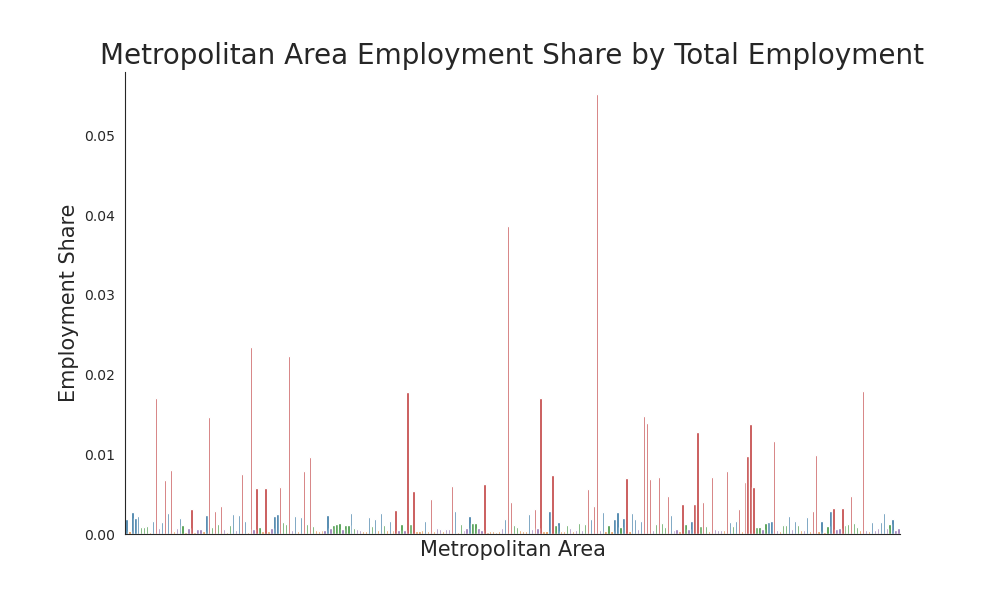
\includegraphics[width=\textwidth]{../../estimations/graphs/city_employment_share.png}
        \subcaption{Employment Share by MSA in 2019}
        \label{employment_city_share}
    \end{minipage}\hfill
    \begin{minipage}{0.48\textwidth}
        \centering
        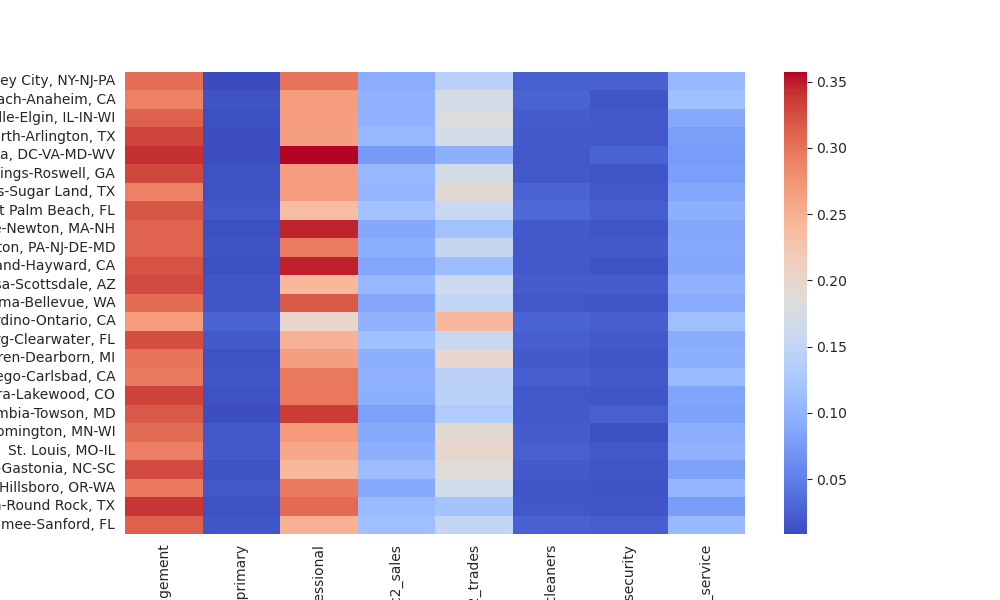
\includegraphics[width=\textwidth]{../../estimations/graphs/top_25_city_heatmap.png}
        \subcaption{Composition of Top 10 MSAs in 2019}
        \label{top_25_city_heatmap}
    \end{minipage}
    \caption*{\small\textit{Note: I will be referring to MSAs as cities throughout the paper. MSAs in Figure \ref{employment_city_share} are arranged in alphabetical order on the x axis.}}
\end{figure}

From the data in Figure \ref{employment_city_share}, I see that a few metropolitan areas own a disproportionate share of employment which illustrates the size effects of cities to attract employment and households. Intuitively, I should expect these cities to be very different from each other in terms of their specialization, otherwise I would expect the largest city with a particular composition to dominate in the share of households. When zooming into the compositions of the top 10 cities however, I see a different story. In Figure \ref{top_25_city_heatmap}, I see that the top 25 cities are very similar with each other in terms of their specialization. With all cities specializing in occupations like management and professional services. While there is some heterogeneity in the composition of cities, the specialization of cities is not as pronounced as I would expect. This indicates to us that the occupation shifter will play a large role in determining the attractiveness of a city.

\subsection{Results}

To recover my$\rho$ parameter, I run a two stage least squares regression with a shift share instrument. I find that this regression yields a high F-Statistic and a significantly higher estimate for $\hat{\beta}$ compared to ols\footnote{Refer to appendix 8.2 for full regression table}. This ultimately results in a fairly high estimate of $\hat{\rho} = 0.67$. The result means that draws across cities within any given occupation id highly correlated and indicates to us that people are very likely to migrate within occupations. This is consistent with the idea that people are more likely to move to cities where they can find jobs in their occupation.

\begin{table}[!htb]
    \centering
    \caption{Estimations for $T_c$ and $T_k$ for 2019}
    \begin{minipage}{0.4\textwidth}
        \centering
        \caption*{(A) Occupation Shifters}
        \begin{tabular}{lr}
\toprule
Occupation & Occupation Shifter \\
\midrule
Management & 0.849566 \\
Professional & 0.743607 \\
Trades & 0.610380 \\
Service & 0.344887 \\
Sales & 0.318461 \\
Cleaners & 0.090246 \\
Primary & 0.066206 \\
Security & 0.066183 \\
\bottomrule
\end{tabular}

    \end{minipage}
    \hfill
    \begin{minipage}{0.55\textwidth}
        \centering
        \caption*{(B) Top City Shifters}
        \begin{tabular}{lr}
\toprule
City & City Shifter \\
\midrule
New York-Newark-Jersey City & 3.029541 \\
Los Angeles-Long Beach-Anaheim & 2.645708 \\
Chicago-Naperville-Elgin & 2.333439 \\
Dallas-Fort Worth-Arlington & 2.158189 \\
Houston-The Woodlands-Sugar Land & 2.093633 \\
Philadelphia-Camden-Wilmington & 2.028458 \\
Washington-Arlington-Alexandria & 2.007037 \\
Atlanta-Sandy Springs-Roswell & 2.001475 \\
\bottomrule
\end{tabular}

    \end{minipage}
    \caption*{\small\textit{Note: Occupation and city shifters are not directly comparable. Recall that occupations are scaled only by $\rho$ while occupations are scaled by $\rho$ and $\theta$. Comparisons should only be relative and be made within each table.}}
\end{table}

In 2019, I find that occupation shifters are generally lower compared to city shifters. However, since cities are scaled by an additional factor of theta, the resulting effect from occupation shifters remains higher than city shifters. For occupation shifters, it's unsurprising that professional and management services have the highest values, given the proportion of households employed in these occupations. Conversely, primary sector occupations have the lowest shifters. Coupled with the fact that these occupations are generally performed in cities with low shifters themselves, this results in cities specializing in primary occupations having low shares of households. It's important to note, however, that while a city-occupation pair may be generally unattractive to most households, those who specialize in these occupations will be very willing to move to cities with occupations matching their abilities.

Most dense metropolitan areas tend to specialize in occupations with high shifters, explaining the large pattern of rural-urban migration to these cities in the past. However, now that most cities have developed similar occupational compositions, I see large cities competing with each other for household shares, which is why no particular city is universally most attractive to all households. While large cities tend to have similar overall compositions, they still manage to distinguish themselves by having distinct compositions in other occupations. For example, although New York may be concentrated in management and professional services, it has a higher concentration in sales compared to Los Angeles. This suggests that these cities are large because of their dominant occupations, but they don't compete purely based on scale with other cities.

Unsurprisingly, cities with the highest shifters are dense metropolitan areas such as New York and Los Angeles, reflecting the large populations they attract. Notable in my estimates is the variance in shifter values between cities, with some shifters being up to three times larger than others, indicating significant heterogeneity in city attractiveness. This makes sense as large cities tend to offer more and better amenities as well as better access to jobs, making them more attractive to households. I also find that city shifters tend to be fairly stable over time, with changes generally below 10\% over the 10-year period. Given the time required for cities to build infrastructure and other amenities, in addition to needing to differentiate themselves from other cities, this stability is not surprising.

\section{Quantitative Exercises}

Using my parameter and shifter estimates, I can now perform two counterfactual exercises. First, I will simulate a city-specific shock to observe migration patterns across cities, focusing on the unbalanced substitution patterns that favor similar cities. Second, I will examine the migration patterns resulting from a shock to a particular occupation. This effectively simulates the effects of a trade shock that impacts some occupations more than others, such as the China shock (\cite{adh2013}). These exercises will provide insights into how different types of economic shocks affect urban migration and occupation choices. In order to perform these exercises, I will assume a parameter $\theta$ of 3 which is an estimate used by \cite{redding} that is obtained from the literature. This will give us my across occupation elasticity.

\subsection{City Specific Shock}

\begin{figure}[!htb]
    \centering
    \caption{Relative Change in City Shares Following New York Shock ($\rho = 0$ vs $\rho = 0.64$)}
    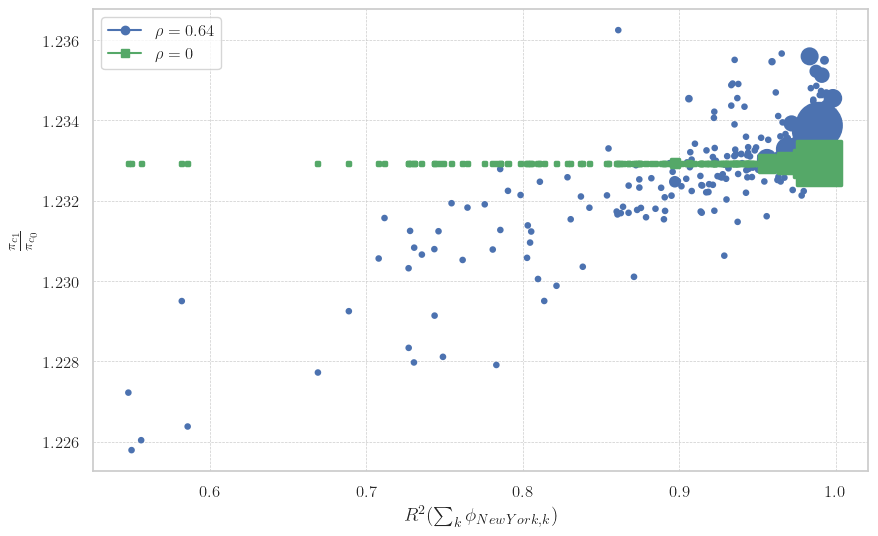
\includegraphics[width=\textwidth]{../../estimations/graphs/city_shock.png}
    \label{ny_change_graph}
    \caption*{\small\textit{Note: The x axis represents the correlation of city compositions of other cities relative to New York. The size of each plot is relative to the size of each city before the negative shock of 5\% to New York. $\pi_{c_0}$ is the city share before the shock, and $\pi_{c_1}$ is the city share after the shock. $\phi_{c, k}$ is the share of occupation $k$ in city $c$. New York is excluded from the plot.}}
\end{figure}

My results from the previous section suggest that while I may observe some migration to large cities purely due to their size, I should expect to see more migration to cities with similar occupational makeups. To test this, I induce a negative shock of 5\% to all occupations in New York, a city primarily focused on management and professional services occupations. The results are shown in Figure \ref{ny_change_graph}.

Analyzing the results, I find that cities benefiting most from this shock have occupational compositions highly correlated with New York, consistent with my previous findings that households are more likely to move to cities with similar occupational compositions. However, city size also plays a significant role in determining migration patterns. At the top end of the correlation, large cities such as Los Angeles and Chicago benefit the most from the New York shock. This suggests that households looking to relocate prefer cities similar to New York, but given the similarity among top cities, the determining factor becomes city size, which in my model correlates perfectly with the benefits each city provides.

Interestingly, when I turn off within-occupation migration by setting $\rho = 0$, the distribution reduces to a standard CES model, as discussed in section 2.1. In this case, households are much more evenly redistributed across cities. With all occupations equally attractive to all households, all cities become perfect substitutes for each other\footnote{Expression \ref{city_cross_elasticity} tells us that the elasticity of each city is governed by $\rho$. When $\rho = 0$, $\sum_{k}^{K} \phi_{c'k} = 1$, all cities will share the same elasticity of $\pi_{c'}.$}.

\begin{figure}[!htb]
    \centering
    \caption{Relative Change in City Shares Following Porterville Shock ($\rho = 0$ vs $\rho = 0.64$)}
    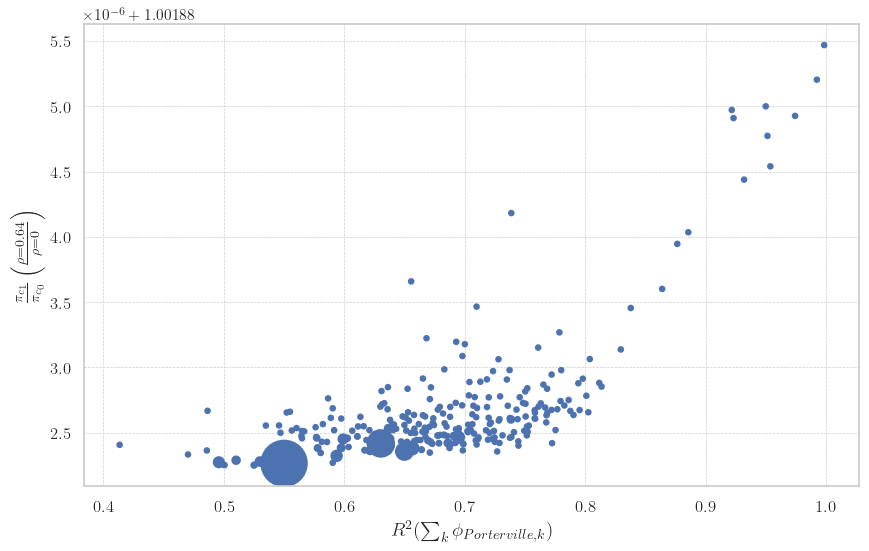
\includegraphics[width=\textwidth]{../../estimations/graphs/city_shock_s.png}
    \label{vp_change_graph}
    \caption*{\small\textit{Note: The x axis represents the correlation of city compositions of other cities relative to Porterville. The size of each plot is relative to the size of each city before the negative shock of 5\% to Porterville. $\pi_{c_0}$ is the city share before the shock, and $\pi_{c_1}$ is the city share after the shock. $\phi_{c, k}$ is the share of occupation $k$ in city $c$. The y axis is the ratio between $\frac{\pi_{c_1}}{\pi_{c_0}}$ when $\rho = 0.64$ and when $\rho = 0$.This ratio was basically flat when $\rho = 0$. The ratio was chosen for the y axis to illustrate the difference in the relative change in city shares when $\rho = 0$ and $\rho = 0.64$. Porterville is excluded from the plot. Note that the scale for the y axis is very small, significantly smaller than the shock to New York.}}
\end{figure}

To further illustrate the importance of occupational composition in migration decisions, I induce a negative shock of 5\% to all occupations in Porterville, a city with a relatively low occupational composition. The results are shown in Figure \ref{vp_change_graph}. I find that the shock to Porterville has a much smaller effect on city shares compared to the shock to New York, which makes sense given it's significantly smaller size. However, the relative change in city shares still remain, with the correlation of occupational composition, or how similar the cities are being the deicing factor for household migration. Here I see that even large cities such as New York will benefit less than smaller cities which have more similar occupations to Porterville. While this is not explicitly illustrated on the figure, I also find that when setting $\rho = 0$, the relative change in city shares is almost identical across all cities, so much so in fact that I started running into limitations in precision when calculating the relative change in city shares for $\rho = 0$.

This exercise illustrates the goal of my model: to better simulate the substitution patterns of households across cities. My findings show that migration patterns are mainly determined by each city's occupational composition. Households are willing to relocate, but primarily to cities offering opportunities in their field. Within the set of cities meeting this criteria, city size becomes the deciding factor. This contrasts with the standard QSM model proposed by \cite{redding}, which would predict that households simply move to the city with the highest amenity value.

\subsection{Occupation Specific Shock}

\begin{figure}[!htb]
    \centering
    \caption{Relative Change in City Shares Following A Shock in Management and Trade Occupations}
    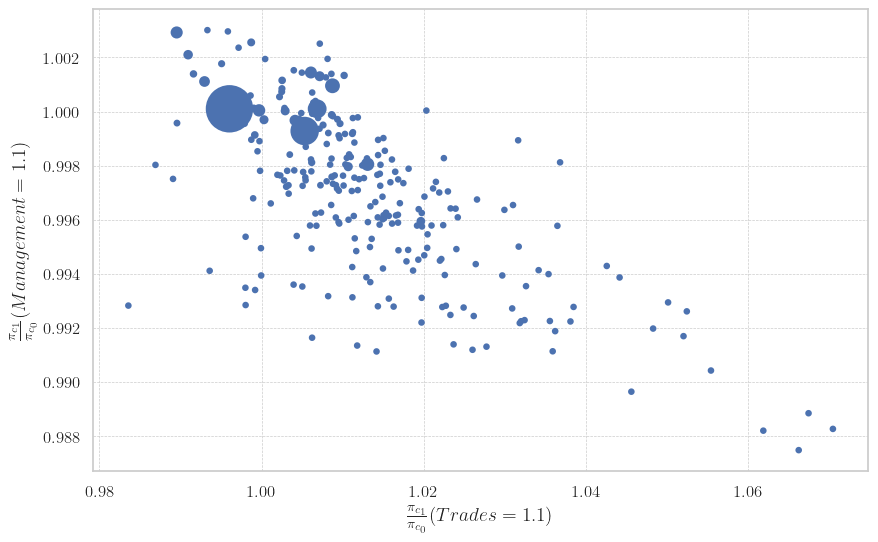
\includegraphics[width=\textwidth]{../../estimations/graphs/occ_shock_t.png}
    \label{man_change_graph}
    \caption*{\small\textit{Note: $\pi_{c_0}$ is the share of households in city $c$ before the positive shock of 10\% to both Management and Primary occupations, and $\pi_{c_1}$ is the share of households in city $c$ after the shock. The size of each plot represents the size of each city before the shock. Both the x and y axis do not start from 1, some cities experience a decrease in the shares of households and some experience an increase. There are also some cities that experience an increase in shares with both shocks.}}
\end{figure}

What happens when there's a shock to particular occupations? We've established that households move to cities with similar occupational profiles when there's a negative shock to specific cities. But how do they respond when a shock affects all cities within a particular occupation? To explore this, I induce a positive shock of 5\% to management and trade occupations across all cities.

Taking a look at the relative change in shares during a shock to management on the y axis of Figure \ref{man_change_graph}, I see that it's mainly the large cities who tend to specialize in these occupations that benefit from the positive shock, while smaller cities that are less concentrated in these occupations tend to lose out. This is consistent with the predictions of my model which states that the effect of a shock on a city is determined by that city's relative concentration in that occupation. When I plot this change against the relative shares following a positive shock to Trade occupations, I get an even clearer picture. Small cities that specialize in trades will benefit from positive shocks to this occupation and lose out when there's a positive shock to management occupations, while the opposite is true for large cities that specialize in management occupations.

Recall Expression \ref{city_occupation_elasticity}, which indicates that the elasticity of a city with respect to an occupation shock is governed by the relative concentration of that occupation in the city. Crucially, this elasticity is not influenced by $\rho$, meaning it should be consistent across different values of $\rho$\footnote{Refer to appendix 8.3 for this figure}. The interpretation is that when there is a shock in cities, households can find employment in the same occupation in other cities, leading to migration to cities with similar compositions. However, when there is a shock in occupations, employment within that given occupation is equally affected across all cities, leading to migration across occupations to cities less affected by the shock. This is exactly what I observe: an even redistribution of households to all other occupations, causing cities that are less concentrated in management occupations to benefit the most from this shock, which, in my case, tend to be smaller cities.

\section{Discussion}

Given the empirical and counterfactual results, I believe there are a couple of important policy implications to consider. Place-based policies that aim to make a city overall more productive in all occupations will generally be ineffective in attracting migration. This is because households tend to pick cities based on their occupations rather than the city itself. A more effective place-based policy should target either occupations that the city already specializes in, or occupations that have a high productivity shifter. Importantly, to increase a city's relative competitiveness, policymakers should focus on occupations that make it less similar to other cities in order to decrease direct competition.

Policies aimed at responding to trade shocks should be focused on transitioning households to other occupations. Unlike city shocks where households can simply move to other cities for better opportunities, trade shocks will result in households being persistently unemployed due to the lack of opportunities in their given occupation specialization. To tackle this form of unemployment, governments need to facilitate the transition of these households to other occupations. This can be done through retraining programs or by providing incentives for firms to hire these workers. Such measures will not only help households find jobs, but will also help cities that are highly specialized in these affected occupations to attract more households. By adopting these targeted approaches, policymakers can more effectively address the challenges posed by both localized economic changes and broader trade shocks, ultimately fostering more resilient urban economies and labor markets.

\section{Conclusion}

In this paper, I have developed a model of city and occupation choice that enables us to recover city and occupation-specific shifters and substitution parameters. My findings demonstrate that occupations play a more significant role in migration decisions compared to cities themselves, with households more likely to relocate to cities with similar occupational compositions. I have also shown that within-occupation migration is more prevalent than across-occupation migration, consistent with the notion that people are more inclined to move to cities where they can find jobs in their current occupation. In the future, I hope to extend this model to include a housing market and unemployment which will allow up to explain housing prices in relatively low productivity cities as well as persistent unemployment in certain cities.

\newpage
\bibliography{latest}

\newpage

\section{Appendix}

\subsection{Derivations}

\noindent\textbf{City Choice Shares $\pi_{c}$}: As discussed in Lind and Ramondo (2023), the choice shares can be expressed as:

\begin{equation*}
    \pi_{c}=\frac{Z_{c}^{-\theta}{G_{c}}}{G()}
\end{equation*}

I define $G()$ as the following, given the definition of $T_{ck}$ and $\lambda_{k}$ provided in the main text:

\begin{equation*}
    G({Z_{1}}^{-\theta},...,{Z_{N}}^{-\theta})=\sum\limits_{k}\Big[\sum\limits_{c}^{N}({T_{ck}}{Z_{c}^{-\theta}})^{\frac{1}{1-\rho_{k}}}\Big]^{1-\rho_{k}} = \sum\limits_{k}{T_{k}}\lambda^{1-\rho}_{k}
\end{equation*}

$G_{c}()$ is simply the derivative of $G()$ with respect to $Z_{c}^{-\theta}$.

\begin{align*}
    \frac{\partial{G()}}{\partial{Z_{c}^{-\theta}}} & = \sum\limits_{k}\frac{\partial}{\partial{Z_{c}^{-\theta}}}\Big[\sum\limits_{c}^{N}({T_{ck}}{Z_{c}^{-\theta}})^{\frac{1}{1-\rho}}\Big]^{1-\rho} \\ &= \sum\limits_{k}\frac{\partial}{\partial{Z_{c}^{-\theta}}}\Big[{T^{\frac{1}{1-\rho}}_{k}}\sum\limits_{c}^{N}({t_{ck}}{Z_{c}^{-\theta}})^{\frac{1}{1-\rho}}\Big]^{1-\rho} \\ &= \sum\limits_{k}{T_{k}}\Big[(1-\rho)\lambda^{-\rho}_{k}\frac{\partial{\lambda_{k}}}{\partial{Z_{c}^{-\theta}}}\Big] \\ &= \sum\limits_{k}{T_{k}}\Big[(1-\rho)\lambda^{-\rho}_{k}(\frac{1}{1-\rho}){t^{\frac{1}{1-\rho}}_{ck}}(Z_{c}^{-\theta})^{\frac{\rho}{1-\rho}}\Big]\\ &= (Z_{c}^{-\theta})^{\frac{\rho}{1-\rho}}\sum\limits_{k}{T_{k}}{t^{\frac{1}{1-\rho}}_{ck}}\lambda_{k}^{-\rho}
\end{align*}

Putting these three terms together, I derive the choice shares:

\begin{align*}
    \pi_{c} & = \frac{Z_{c}^{-\theta}{G_{c}}}{G()} \\ &= (Z_{c}^{-\theta})^{\frac{1}{1-\rho}}\Bigg[\frac{\sum\limits_{k}{t^{\frac{1}{1-\rho}}_{ck}}{T_{k}}\lambda_{k}^{-\rho}}{\sum\limits_{k}{T_{k}}\lambda_{k}^{1-\rho}}\Bigg]
\end{align*}

\noindent\textbf{Own Occupation-Specific Elasticity:} I wish to evaluate $\partial\ln{\pi_{c}}/\partial\ln{t_{ck}}$, under the assumption that $\partial\ln{\lambda_{k}}/\partial\ln{t_{ck}}=0$. Notice this assumption yields the following:

\begin{equation*}
    \frac{\partial\ln{\pi_{c}}}{\partial\ln{t_{ck}}} \approx \frac{\partial\ln{\pi_{ck}}}{\partial\ln{t_{ck}}} - \frac{\partial\ln{\phi_{ck}}}{\partial\ln{t_{ck}}}
\end{equation*}

given the definitions of $\pi_{ck}$ and $\phi_{ck}$ provided in the text.

Notice that this only leaves one term to evaluate if I take the logarithm of $\pi_{c}$ and the derivative of this logarithm with respect to $\ln{t_{ck}}$:

\begin{align*}
    \frac{\partial\ln{\pi_{c}}}{\partial\ln{t_{ck}}} & \approx \frac{\partial\ln[{\sum\limits_{k}{t^{\frac{1}{1-\rho}}_{ck}}{T_{k}}\lambda_{k}^{-\rho}}]}{\partial\ln{t_{ck}}} \\ &= \Bigg(\frac{\partial[{\sum\limits_{k}{t^{\frac{1}{1-\rho}}_{ck}}{T_{k}}\lambda_{k}^{-\rho}}]}{\partial{t_{ck}}}\Bigg)\Bigg(\frac{t_{ck}}{{\sum\limits_{k}{t^{\frac{1}{1-\rho}}_{ck}}{T_{k}}\lambda_{k}^{-\rho}}}\Bigg)\\ &= \Bigg(\frac{1}{1-\rho}\Bigg)\Bigg(\frac{t_{ck}^{\frac{1}{1-\rho}}{T_{k}}\lambda_{k}^{-\rho}}{t_{ck}}\Bigg)\Bigg(\frac{t_{ck}}{{\sum\limits_{k}{t^{\frac{1}{1-\rho}}_{ck}}{T_{k}}\lambda_{k}^{-\rho}}}\Bigg) \\ &= \Big(\frac{1}{1-\rho}\Big)\Bigg[\frac{{t^{\frac{1}{1-\rho}}_{ck}}{T_{k}}\lambda_{k}^{-\rho}}{\sum\limits_{k}{t^{\frac{1}{1-\rho}}_{ck}}{T_{k}}\lambda_{k}^{-\rho}}\Bigg]\\ &= \frac{\phi_{ck}}{1-\rho}
\end{align*}

\noindent\textbf{Cross-City Occupation-Specific Elasticity:} I wish to evaluate $\partial\ln{\pi_{c}}/\partial\ln{t_{{c'}k}}$. Notice that this elasticity can be expressed as the following two terms:

\begin{equation*}
    \frac{\partial\ln{\pi_{c}}}{\partial\ln{t_{{c'}k}}} = {t^{\frac{1}{1-\rho}}_{ck}}{T_{k}}\Big(\frac{\partial\lambda_{k}^{-\rho}}{\partial{t_{{c'}k}}}\Big)\Big(\frac{t_{{c'}k}}{{\sum\limits_{k}{t^{\frac{1}{1-\rho}}_{ck}}{T_{k}}\lambda_{k}^{-\rho}}}\Big) - {T_{k}}\Big(\frac{\partial\lambda_{k}^{1-\rho}}{\partial{t_{{c'}k}}}\Big)\Big(\frac{t_{{c'}k}}{{\sum\limits_{k}{T_{k}}\lambda_{k}^{1-\rho}}}\Big)
\end{equation*}

It will be useful to first define the derivative of $\lambda_{k}$ with respect to myvariable of interest, $t_{{c'}k}$:

\begin{equation*}
    \frac{\partial{\lambda_{k}}}{\partial{t_{{c'}k}}} = \Big(\frac{1}{1-\rho}\Big)\Big(\frac{1}{t_{{c'}k}}\Big)[{t_{{c'}k}}(Z_{c'}^{-\theta})]^{\frac{1}{1-\rho}}
\end{equation*}

I can now use chain rule in order to evaluate my elasticity of interest. The first term becomes the following:

\begin{align*}
    {t^{\frac{1}{1-\rho}}_{ck}}{T_{k}}\Big(\frac{\partial\lambda_{k}^{-\rho}}{\partial{t_{{c'}k}}}\Big)\Big(\frac{t_{{c'}k}}{{\sum\limits_{k}{t^{\frac{1}{1-\rho}}_{ck}}{T_{k}}\lambda_{k}^{-\rho}}}\Big) & = {t^{\frac{1}{1-\rho}}_{ck}}{T_{k}}(-\rho)(\lambda_{k}^{-\rho-1})\Big(\frac{1}{1-\rho}\Big)\Bigg(\frac{[{t_{{c'}k}}(Z_{c'}^{-\theta})]^{\frac{1}{1-\rho}}}{{\sum\limits_{k}{t^{\frac{1}{1-\rho}}_{ck}}{T_{k}}\lambda_{k}^{-\rho}}}\Bigg) \\ &= -\Bigg(\frac{\rho}{1-\rho}\Bigg)\Bigg(\frac{[{t_{{c'}k}}(Z_{c'}^{-\theta})]^{\frac{1}{1-\rho}}}{\lambda_{k}}\Bigg)\Bigg(\frac{t^{\frac{1}{1-\rho}}_{ck}{T_{k}}{\lambda^{-\rho}_{k}}}{{\sum\limits_{k}{t^{\frac{1}{1-\rho}}_{ck}}{T_{k}}\lambda_{k}^{-\rho}}}\Bigg)\\ &= -\Bigg(\frac{\rho}{1-\rho}\Bigg)\Bigg(\frac{[{t_{{c'}k}}(Z_{c'}^{-\theta})]^{\frac{1}{1-\rho}}}{\lambda_{k}}\Bigg){\phi_{ck}}\\ &= -\Big(\frac{\rho}{1-\rho}\Big){\pi_{{c'}k}}{\phi_{ck}}
\end{align*}

The second term can be derived in the following way:

\begin{align*}
    - {T_{k}}\Big(\frac{\partial\lambda_{k}^{1-\rho}}{\partial{t_{{c'}k}}}\Big)\Big(\frac{t_{{c'}k}}{{\sum\limits_{k}{T_{k}}\lambda_{k}^{1-\rho}}}\Big) & = - {T_{k}}(\lambda_{k}^{-\rho})[{t_{{c'}k}}(Z_{c'}^{-\theta})]^{\frac{1}{1-\rho}}\Big(\frac{1}{{\sum\limits_{k}{T_{k}}\lambda_{k}^{1-\rho}}}\Big) \\ &= - \Bigg(\frac{[{t_{{c'}k}}(Z_{c'}^{-\theta})]^{\frac{1}{1-\rho}}}{\lambda_{k}}\Bigg)\Big(\frac{{T_{k}}{\lambda_{k}^{1-\rho}}}{{\sum\limits_{k} T_k \lambda_{k}^{1-\rho}}}\Big)\\ &= -\pi_{{c'}k}{\omega_{k}}
\end{align*}

Putting these together, I derive the cross-city occupation-specific elasticity as the following:

\begin{equation*}
    \frac{\partial\ln{\pi_{c}}}{\partial\ln{t_{{c'}k}}} = -{\pi_{{c'}k}}\Big[\omega_{k}+\Big(\frac{\rho}{1-\rho}\Big)\phi_{ck}]
\end{equation*}

Notice that this is equivalent to the following, given the identity linking $\pi_{c}$, $\pi_{ck}$, $\phi_{ck}$, and $\omega_{k}$.

\begin{equation}
    \frac{\partial\ln{\pi_{c}}}{\partial\ln{t_{{c'}k}}} = -{\pi_{c'}}{\phi_{ck}}\Big[1+\Big(\frac{\rho}{1-\rho}\Big)\Big(\frac{\pi_{ck}}{\pi_{c}}\Big)\Big]
\end{equation}

\noindent\textbf{Cross-City Aggregate Elasticity:} I wish to evaluate $\partial\ln{\pi_{c}}/\partial\ln{T_{c'}}$. Notice that:

\begin{equation*}
    \frac{\partial\ln{\pi_{c}}}{\partial\ln{T_{c'}}} = \Bigg(\frac{\sum\limits_{k}{{t^{\frac{1}{1-\rho}}_{ck}}}{T_{k}}{\lambda^{-\rho}_{k}}}{\partial{T_{c'}}}\Bigg)\Bigg(\frac{T_{c'}}{\sum\limits_{k}t^{\frac{1}{1-\rho}}_{ck}{T_{k}}{\lambda^{-\rho}_{k}}}\Bigg) - \Bigg(\frac{\partial\sum\limits_{k}{T_{k}}\lambda^{1-\rho}_{k}}{\partial{T_{c'}}}\Bigg)\Bigg(\frac{T_{c'}}{\sum\limits_{k}{T_{k}}{\lambda_{k}^{1-\rho}}}\Bigg)
\end{equation*}

Notice also that:

\begin{equation*}
    \frac{\partial\lambda_{k}}{\partial{T_{c'}}} = \Bigg(\frac{1}{1-\rho}\Bigg)\Bigg(\frac{[t_{ck}(Z_{c}^{-\theta})]^{\frac{1}{1-\rho}}}{T_{c'}}\Bigg)
\end{equation*}

I can therefore solve for this cross-derivative as the following:

\begin{align*}
    \frac{\partial\ln{\pi_{c}}}{\partial\ln{T_{c'}}} & = \sum\limits_{k}\Big[-\Big(\frac{\rho}{1-\rho}\Big)\phi_{ck}{\pi_{{c'}k}}\Big]+\sum\limits_{k}\Big[-\omega_{k}\pi_{{c'}k}\Big] \\ &= -\sum\limits_{k}{\pi_{{c'}k}}\Big[\omega_{k}+\Big(\frac{\rho}{1-\rho}\Big)\phi_{ck}\Big]
\end{align*}

\subsection{Regression Tables}

\subsubsection{First Stage Shift Share Regression}
\begin{table}[!htbp] \centering
\begin{tabular}{@{\extracolsep{5pt}}lc}
\\[-1.8ex]\hline
\hline \\[-1.8ex]
& \multicolumn{1}{c}{\textit{Dependent variable: wage}} \
\cr \cline{2-2}
\\[-1.8ex] & (1) \\
\hline \\[-1.8ex]
 sim\_wage & 0.523$^{***}$ \\
& (0.037) \\
\hline \\[-1.8ex]
 Observations & 19280 \\
 $R^2$ & 0.881 \\
 Adjusted $R^2$ & 0.863 \\
 Residual Std. Error & 0.198 (df=16799) \\
 F Statistic & 3696120.683$^{***}$ (df=2480; 16799) \\
\hline
\hline \\[-1.8ex]
\textit{Note:} & \multicolumn{1}{r}{$^{*}$p$<$0.1; $^{**}$p$<$0.05; $^{***}$p$<$0.01} \\
\end{tabular}
\end{table}

\newpage

\subsubsection{OLS vs IV Regression}
\begin{table}[!htbp] \centering
    \caption{Estimates Of The Effect Of Wages On City Shares With City And Occupation Fixed Effects}
    \begin{tabular}{@{\extracolsep{5pt}}lcc}
        \\[-1.8ex]\hline
        \hline                                                                                        \\[-1.8ex]
                    & \multicolumn{2}{c}{\textit{Dependent variable: City Shares}} \
        \cr \cline{2-3}
        \\[-1.8ex] & \multicolumn{1}{c}{OLS} & \multicolumn{1}{c}{IV}  \\
        \\[-1.8ex] & (1) & (2) \\
        \hline                                                                                        \\[-1.8ex]
        Wage        & 0.291$^{***}$                                                   &               \\
                    & (0.023)                                                         &               \\
                    &                                                                 & 2.777$^{***}$ \\
                    &                                                                 & (0.041)       \\
        \hline                                                                                        \\[-1.8ex]
        $R^2$       & 0.956                                                           &               \\
        F Statistic &                                                                 & 145.8$^{***}$ \\
        \hline
        \hline                                                                                        \\[-1.8ex]
        % \textit{Note:} & \multicolumn{2}{r}{$^{*}$p$<$0.1; $^{**}$p$<$0.05; $^{***}$p$<$0.01}                   \\
    \end{tabular}
    \caption*{\small\textit{Note: This is the results of the regression using the estimation equation discussed in section 3.1. All city and occupation fixed effects are omitted for brevity. Standard errors are clustered on city-occupation pairs and are in parenthesis. $^{*}$p$<$0.1; $^{**}$p$<$0.05; $^{***}$p$<$0.01}}
    \label{city_sec_iv_ols}
\end{table}

\newpage

\subsection{Figures}

\begin{figure}[!htb]
    \centering
    \caption{Relative Change in City Shares Following A Shock in Management ($\rho = 0$ vs $\rho = 0.64$)}
    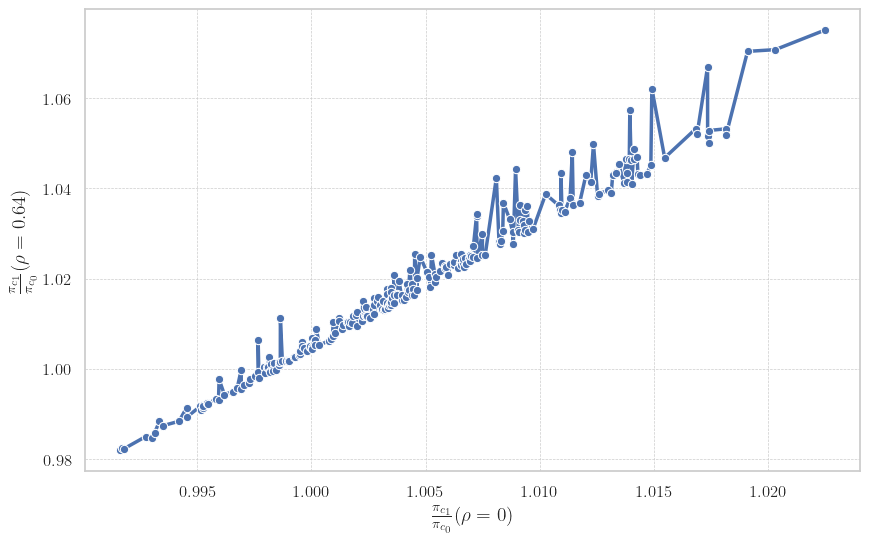
\includegraphics[width=\textwidth]{../../estimations/graphs/occ_shock.png}
    \caption*{\small\textit{Note: $\pi_{c_0}$ is the share of households in city $c$ before the negative shock of 5\% to Management occupations, and $\pi_{c_1}$ is the share of households in city $c$ after the shock. The size of each plot represents the size of each city before the shock. Both the x and y axis do not start from 1, some cities experience a decrease in the shares of households and some experience an increase.}}
\end{figure}

\end{document}